%%
%% This is file `sigconf.tex',
%% generated with the docstrip utility.
%%
%% The original source files were:
%%
%% samples.dtx  (with options: `all,proceedings,sigconf')
%% 
%% IMPORTANT NOTICE:
%% 
%% For the copyright see the source file.
%% 
%% Any modified versions of this file must be renamed
%% with new filenames distinct from sigconf.tex.
%% 
%% For distribution of the original source see the terms
%% for copying and modification in the file samples.dtx.
%% 
%% This generated file may be distributed as long as the
%% original source files, as listed above, are part of the
%% same distribution. (The sources need not necessarily be
%% in the same archive or directory.)
%%
%%
%% Commands for TeXCount
%TC:macro \cite [option:text,text]
%TC:macro \citep [option:text,text]
%TC:macro \citet [option:text,text]
%TC:envir table 0 1
%TC:envir table* 0 1
%TC:envir tabular [ignore] word
%TC:envir displaymath 0 word
%TC:envir math 0 word
%TC:envir comment 0 0
%%
%% The first command in your LaTeX source must be the \documentclass
%% command.
%%
%% For submission and review of your manuscript please change the
%% command to \documentclass[manuscript, screen, review]{acmart}.
%%
%% When submitting camera ready or to TAPS, please change the command
%% to \documentclass[sigconf]{acmart} or whichever template is required
%% for your publication.
%%
%%
\documentclass[nonacm,sigconf]{acmart}
\usepackage{tabularx}
\usepackage{listings}

%%
%% \BibTeX command to typeset BibTeX logo in the docs
\AtBeginDocument{%
  \providecommand\BibTeX{{%
    Bib\TeX}}}

%% Rights management information.  This information is sent to you
%% when you complete the rights form.  These commands have SAMPLE
%% values in them; it is your responsibility as an author to replace
%% the commands and values with those provided to you when you
%% complete the rights form.

%% These commands are for a PROCEEDINGS abstract or paper.
%%
%%  Uncomment \acmBooktitle if the title of the proceedings is different
%%  from ``Proceedings of ...''!
%%
%%\acmBooktitle{Woodstock '18: ACM Symposium on Neural Gaze Detection,
%%  June 03--05, 2018, Woodstock, NY}


%%
%% Submission ID.
%% Use this when submitting an article to a sponsored event. You'll
%% receive a unique submission ID from the organizers
%% of the event, and this ID should be used as the parameter to this command.
%%\acmSubmissionID{123-A56-BU3}

%%
%% For managing citations, it is recommended to use bibliography
%% files in BibTeX format.
%%
%% You can then either use BibTeX with the ACM-Reference-Format style,
%% or BibLaTeX with the acmnumeric or acmauthoryear sytles, that include
%% support for advanced citation of software artefact from the
%% biblatex-software package, also separately available on CTAN.
%%
%% Look at the sample-*-biblatex.tex files for templates showcasing
%% the biblatex styles.
%%
%%
%% The majority of ACM publications use numbered citations and
%% references.  The command \citestyle{authoryear} switches to the
%% "author year" style.
%%
%% If you are preparing content for an event
%% sponsored by ACM SIGGRAPH, you must use the "author year" style of
%% citations and references.
%% Uncommenting
%% the next command will enable that style.
%%\citestyle{acmauthoryear}


%%
%% end of the preamble, start of the body of the document source.
\begin{document}

%%
%% The "title" command has an optional parameter,
%% allowing the author to define a "short title" to be used in page headers.
\title{Hacker News vs Google: how do specialised topic trends compare?}

%%
%% The "author" command and its associated commands are used to define
%% the authors and their affiliations.
%% Of note is the shared affiliation of the first two authors, and the
%% "authornote" and "authornotemark" commands
%% used to denote shared contribution to the research.
\author{Thomas De Noronha Tomei}
\email{thomas.tomei@colorado.edu}
\affiliation{%
  \city{London}
  \country{United Kingdom}
}

%%
%% By default, the full list of authors will be used in the page
%% headers. Often, this list is too long, and will overlap
%% other information printed in the page headers. This command allows
%% the author to define a more concise list
%% of authors' names for this purpose.
\renewcommand{\shortauthors}{T. Tomei}

%%
%% The abstract is a short summary of the work to be presented in the
%% article.
\begin{abstract}
    In this project, we aim to explore the trends of topics that occurred in Hacker News from its inception in 2006 to present day and compare it with data on related keywords from Google search using Google trends. The goal is to observe whether a specialised community has different trend patterns than the more general population of internet users (represented by Google)
    \par
    We want to understand patterns in the trends in comparison with each other. For instance, if the high popularity of a particular subject coincides between the two sources, or do we have one of the sources starting to notice a topic earlier than the other. Or if topics endure in one website versus the other. Finally, we'd like to understand if any topics are too niche to barely account for Google attention, or if the volume of attention is consistent between platforms
\end{abstract}

%% Removes the ACM reference format (https://tex.org.uk/macros/latex/contrib/acmart/acmart.pdf)
\settopmatter{printacmref=false}

%%
%% This command processes the author and affiliation and title
%% information and builds the first part of the formatted document.
\maketitle


\section{Introduction}
Hacker News is a social news website run by YC combinator, a Silicon Valley startup accelerator and investment fund\footnote{https://news.ycombinator.com/newsguidelines.html}. Much like its owner, the website skews towards topics in computer science and entrepreneurship. It allows users to publish stories, to comment on those, and to upvote/downvote either. It also has functionality for users to post jobs and polls, but those will be excluded from the analysis to simplify the analysis. Google needs no introduction, it's the world's most used search engine. The methodology for what counts as a search is varied, but it is estimated to be 80-90\% over the past 15 years, and it already holds the top spot in 2006\footnote{https://gs.statcounter.com/search-engine-market-share\#monthly-200901-202607} \footnote{https://www.fool.com/investing/general/2013/05/20/google-stock-buy-it-and-hold-it-for-life.aspx}, when Hack That makes it a suitable proxy for the average internet user.
\par
In this project, we examine the trends in topics from Hacker News over time and compare them to the the same topic's keywords from Google trends. This is to understand how much awareness the general population has over time on specialised topics; how much is the delay, if any, between it enters the general population's awareness, and what kind of correlation we have for the metrics of popularity in Hacker News and wider spread popularity. We believe this helps understand information gaps between the two populations, help pinpoint examples that widespread awareness was faster, which can encourage the study of what factors led to such awareness.
\par
For this analysis, we start by clustering articles per topic and scoring them on interaction to quantify how much attention each topic has gathered over time; for each topic, we extract relevant keywords and we analyse the volume of the group of keywords over time. Finally, we compare the trends between the two sources and extract statistics to compare the distributions. For the most popular Hacker News topics, we plot them side-by-side with the Google distribution using a min-max normalisation since it's likely that engagement is not going to be equivalent to search impressions in volume.

\section{Related Work}
The work for this project intersects a couple of more commonly explored topics: usage of Hacker News data for different enquiries, techniques for analysing social media data and topic extraction.

\subsection{Hacker News studies}

Potter \cite{potterhackernews} came the closest to replicating the experiment setting that we're attempting. He has cherry picked 15 topics from Hacker News and plotted them against Google Trends. He hasn't published his methodology, but has linked the dataset\footnote{https://www.kaggle.com/datasets/santiagobasulto/all-hacker-news-posts-stories-askshow-hn-polls} he used. Barik et al \cite{barik15} used Hacker News data to use in grounded theory research on the experience of software engineers. The idea was to pose relevant queries against the data (e.g. "What makes a great software engineer?" or "What are the practices of agile teams?") and extract posts or comments relevant to the question. They note that this technique was successfully implemented on StackOverflow and GitHub. They used simple searches against the platform. Aniche et al \cite{aniche18} interviewed top contributors and analysed post contents to understand the motivations of contributors in online developer communities. Their aim was to improve best practices and tooling for those. The analysis is done mostly in manual reviews of content. Geng et al \cite{geng16} runs different techniques for topic modelling and classifiers on Hacker News's datasets in an attempt to predict post popularity scores. Kraishan \cite{kraishan25} uses the dataset to understand the impact of social news platforms on launch for open-source projects, correlating well-timed exposure of projects within Hacker News with GitHub star counts. The project goes into more detail on other relevant factors, such as post timing. Miklian et al \cite{miklian26} examines veracity of accusations of AI-generated content for forum comments. They have used LLMs to judge the content and calculate the accuracy of each type of accusation. Churchill and Singh \cite{churchill21} focus on preprocessing of social media text to improve downstream processing by reducing noise, and test their results in some datasets, including Hacker News. Finally, Stoddard \cite{stoddard15} studies whether social news aggregator promotes the best content, and what other factors intervene.

\subsection{Analysis of social media and topic extraction}

Topic extraction in social media has been widely researched. Nanayakkara et al \cite{Nanayakkara24} conducted a review of three different methods for extraction of topic: Bidirectional Encoder Representations from
Transformers (BERTopic), Non-negative Matrix Factorisation (NMF) and Latent Dirichlet Allocation (LDA). They used the Youtube dataset for the analysis, and common python libraries like SKLearn\footnote{https://scikit-learn.org/stable/} and Genism\footnote{https://radimrehurek.com/gensim/}. Hankar et al \cite{Hankar25} engage in a review of topic modelling techniques. It offers a wide variety of methodologies and applications, and concludes that, for text classification, BERTopic tends to have improved results. Balaji et al \cite{balaji21} have a wider review of machine learning methods used in social media analysis. Panpan et al \cite{panpan13} develop a visualisation for topic competition to understand how it sets the public agenda, and uses Apache Lucene\footnote{https://lucene.apache.org/} to index and search the raw data. Topics were preset with the help of experts and Twitter hashtags.

\subsection{Our contribution}

We build on the existing work by comparing the dataset from a specialised community and Google trends with a clustering algorithm for topic extraction. We leverage existing already-mentioned techniques for dataset pre-processing and topic extraction for Hacker News and Google trends, so we can obtain two comparable normalised distributions. We would like to understand the general behaviour of the distributions and drivers of similarity / differences.

\section{Proposed work}
\begin{figure}
    \centering
    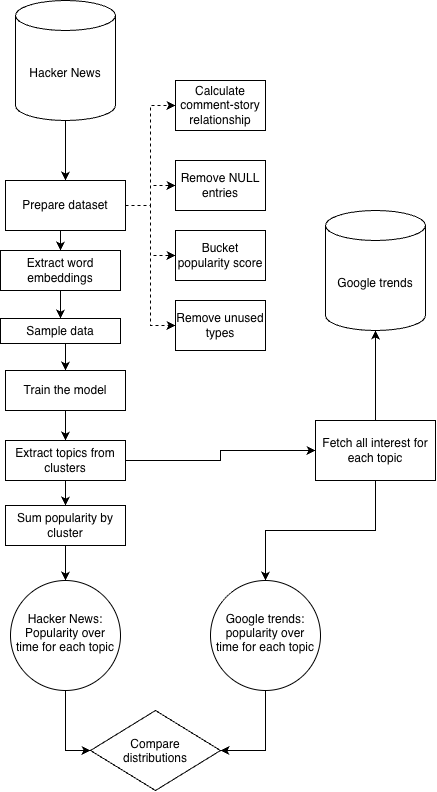
\includegraphics[width=0.9\linewidth]{Data pipeline checkpoint.png}
    \caption{End-to-end flow for the data processing needed to be able to compare Hacker News and Google trend topic popularity}
    \label{fig:pipeline_overview}
    \Description{Dataflow is: fetch data from Hacker News, prepare and preprocess it, then cluster into topics and calculate the populate. For each topic, generate most relevant keywords and fetch interest from Google trends. Finally, compare the two distributions}
\end{figure}

\subsection{Datasets}

Both datasets are available for free. Hacker News has a BigQuery table with all its data from its inception in 2006. The dataset is a single table, \texttt{bigquery-public-data.hacker\_news}. On Aug 15,2026, it had 49,249,015 rows. It contains the following fields described in Table \ref{tab:hackernews}. As you can see, the dataset makes no differentiation between a story row, a comment row and other types of rows. Furthermore, there are plenty of rows with dead stories (i.e. links that don't work or stories/comments that have been deleted) and rows almost entirely made out of NULL.

\begin{table*}[htbp]
    \begin{tabular}{p{0.1\linewidth}|p{0.7\linewidth}|p{0.2\linewidth}}
         Column name & Description & Value type  \\
         \hline
         title & Required for story, job, and poll. Always absent for comment. & Free-form text \\ 
         url & Points to a URL on the internet. Can be associated with text, but doesn't need to be. & NULL, or url \\
         text & Story text (optional). & NULL or free form text \\
         dead & Whether the link, story or post is dead. & NULL or true \\
         by & Username of the poster. & NULL or username \\
         score & Upvotes for a particular story or poll. Always NULL for comments. & NULL or integer (can be -1) \\
         time & Unix time (always present when timestamp is present). & NULL or integer \\
         timestamp & Unix timestamp (always present when time is present). & NULL or datetime \\
         type & Type of content. & One of (job, story, comment, pollopt, poll) \\
         id & ID of the content, can be referenced with https://news.ycombinator.com/item?id=<id>. Unique identifier & Integer \\
         parent & Used to identify what story/comment/poll a comment is linked to. Always NULL for stories. & Existing id \\
         descendants & Count of descendants for a story or poll. Always NULL for comments. & NULL or integer (can be -1) \\
    \end{tabular}
    \caption{Hacker News dataset description}
    \label{tab:hackernews}
\end{table*}

Google trends has a website that you can input up to 5 keywords and analyse a normalised distribution. When you input the keywords, it's going to give you the relative distributions between the topics, with the maximum interest of all the topic being 100 (and the minimum being 0). Because of this normalisation, to understand the relative volume of the data between different queries, we'll need one or more control keywords that have to be carefully chosen to make sure that, once we scale that, we're able to compare two different queries.

\subsection{Data preparation}

The steps for data preparation are as follows:

\begin{itemize}
    \item Remove invalid / uninteresting rows
    \item Resolve story-comment relationship
    \item Assemble the full document
    \item Compute the popularity for an individual story
\end{itemize}

The original dataset was in BigQuery, so we decided to leverage BigQuery itself to all computations we possibly could, given its superior parallelism to what can be obtained in a single-worker (even if multiprocessing / multithreading) colab notebook. BigQuery was also used for all of the data warehousing of the project.

\paragraph{Remove invalid / uninteresting rows} The dataset has a lot of rows that contain NULLs, dead stories, job postings, polls and pollopt (i.e. poll options), and comments that reference any of those. We're not interested in any rows outside of stories and comments. We want to leave the table with only valid stories and comments that can be traced back to stories. We created two views for the data initially, \texttt{hackernews\_story} and \texttt{hackernews\_comment} as further understood the data and what fields were relevant for each of the entities.
\paragraph{Resolve story-comment relationship} Upon further inspection of the dataset, we noticed comments could have a tree structure, as opposed to linking directly to the story (and the story was the root of the tree). We need to do a tree traversal to link stories and comments.
\paragraph{Assemble the full document} We want to have, for each story, the id, title, the free form text, and a concatenation of the text of all the comments. We included timestamps for each of the comments and also the story publication. Finally, we want the story score to be able to calculate the overall score.
\paragraph{Compute the popularity for an individual story} We're defining the population of a story by the sum of votes it gets and the count of comments. It's worth noting, though, that comments can happen way later in time, and because we have a timestamp for them, we can add the comment to the correct bucket. For instance, let's suppose that a story was published March 30th, it received 50 votes overall, then received two comments that day, then 2 more on April 2nd. Here's how the popularity distribution for that story would look like:

\begin{verbatim}
    (0001 // story id, 2026-03-30, 52)
    (0001 // story id, 2026-04-02, 2)
\end{verbatim}

This is not a perfect measure of engagement. We acknowledge that, because of the score of a story / comment being upvotes minus downvotes, it will be a floor to how many votes it got. Another simplification on the temporal aspect of popularity was that it's likely that points are more distributed that the initial publication of the story. However, because Google trends data is bucketed by month when you request all-time data, the granularity of the bucket makes this problem way less apparent than it would have been for a day-bucketed distribution. For the full dataset, 4.6 million stories are contained to a month, 74,000 live two months, and less than 200 live more than that.

At the end we should have transformed the data into Table \ref{tab:cleaned}. Because we might end up with a significant amount of text (the data set has about 5 million story, and about 42 million comments, and the free form text fields are of arbitrary length), we want to save those to a data warehouse to prevent recomputation once we're happy with the new schema and then stream them to the next step of the algorithm.

\begin{table*}[htbp]
  \caption{Hacker News schema after preparation steps}
  \label{tab:cleaned}
  \begin{tabular}{cl}
    Column name&Description\\
    \hline
    story\_id & Original story ID. \\
    story\_link & A url in the format https://news.ycombinator.com/item?id=<id>. \\
    story\_score & The original story score. 0 if NULL. \\
    story\_timestamp & Timestamp for the story's initial publication. \\
    story\_title & Unmodified title. \\
    story\_text & Unmodified story text. "" if NULL. \\
    comments\_text & Concatenation of the texts of all comments. "" if the comment has NULL value. "" if the story has no comments. \\
    comments\_ids & Array with all comment ids that are linked to this story. \\
    comments\_timestamps & Array with all timestamps from comments linked to this story. \\
\end{tabular}
\end{table*}

\subsection{Pre-processing and clustering}

According to the review of the literature, there are many routes that can be taken. The most commonly used algorithm for this analysis would LDA, which is implemented in popular libraries like the aforementioned SKLearn and Gensim. BERTopic is also made available on GitHub\footnote{https://maartengr.github.io/BERTopic/index.html} to be used in a Jupyter notebook. As a starting point, we'll use the clustering tutorial from Dimensions.ai\footnote{https://www.dimensions.ai/products/all-products/dimensions-on-google-bigquery/}, which leverages native BigQuery functionalities to cluster the data\footnote{https://bigquery-lab.dimensions.ai/tutorials/05-topic\_clusters/}. The tutorial uses the Universal Sentence Encoder\footnote{https://www.kaggle.com/models/google/universal-sentence-encoder}, first presented in Cer et al \cite{DBLP:journals/corr/abs-1803-11175}, which compares positively with other embedding methods due to pre-training.

For the clustering algorithm, we used k-means. We're aware that k-means is likely to underperform other algorithms, as the related work section pointed out. However, due to timeline constraints and its availability in BigQuery ML as a potential model \footnote{https://docs.cloud.google.com/bigquery/docs/reference/standard-sql/bigqueryml-syntax-create-kmeans}, it is our model of choice. To attempt to mitigate not leaning into the state of the art for clustering, we'll calibrate its number of clusters with several trials with different parameters \footnote{https://docs.cloud.google.com/bigquery/docs/reference/standard-sql/bigqueryml-syntax-create-kmeans\#hyperparameter\_tuning}

\subsection{Topic extraction and popularity}

Once we have the topics extracted, it is trivial to perform a scan of the dataset and obtain the popularity per topic, it's the sum of the popularity of all the articles in the cluster for a timestamp. That will give us a distribution of popularity per topic over time. To be able to compare with search trends data, the final step is to normalise all the distributions.

\subsection{Google trends distribution}

The algorithm from the tutorial above already comes up with a set of concepts that's associated with a cluster, which makes it not necessary to generate any keywords. We can simply use the concepts outlined. However, as mentioned in the dataset description, we need baseline keyword(s) so we retain our ability to compare different distributions in volume. We propose comparing keywords pairwise and sorting them according to the mid-range of each distribution so they're not too distant from each other and can still provide meaningful values when compared.

After sorting, we can pick up two adjacent distributions (A, B) and (B, C), where mid-range(A) < mid-range(B). We can use the change in scale of B to infer the relationship from A to C. Once we do that for all the distributions, we'll have all distributions on the same scale. We then sum the keywords for the same topic and finally, we normalise them so all the values in all distributions are within the range [0, 1]. That allows us to compare those with the Hacker News topic distributions.

\section{Evaluation}

\paragraph{Distribution plotting per topic} Given distributions are all two-dimensional, and we're using k-means, which allows us to set the number of topics we're looking at, we can perform a visual analysis of both distributions.

\paragraph{Clustering quality metrics} To help choose a sensible k that we can still analyse with plotting the graphs for each topic, we want to tune k so it offers diminishing returns on intra and inter cluster distances. We opted to use the Davies-Bouldin index\footnote{https://en.wikipedia.org/wiki/Davies-Bouldin\_index}, which captures a relationship between exactly those metrics.

We ran our clustering algorithm for 9 trials with different numbers of clusters (k), using the Davies-Bouldin index to contrast performance. The results are in Table \ref{tab:kmeansbest}, which is sorted from lowest to highest index, and clearly demonstrates that k=3 achieves the best performance.

\begin{table}[h]
  \caption{k-means trial results}
  \label{tab:kmeansbest}
  \begin{tabular}{|c|c|c|}
    \hline
    ID & Number of clusters&Davies-Bouldin index\\
    \hline
    4 & 3.0000 & 2.1001 \\
    5 & 2.0000 & 2.5246 \\
    3 & 5.0000 & 4.4259	\\
    1 & 6.0000 & 4.6467 \\
    8 & 8.0000 & 4.7129 \\
    2 & 7.0000 & 4.7764	\\
    6 & 10.0000	& 5.4605 \\
    7 & 9.0000 & 5.4866	\\
    9 & 4.0000 & 5.5879 \\
    \hline
\end{tabular}
\end{table}

\paragraph{Clustering efficiency} The clustering processing is the heaviest part of the processing for the project, so as a secondary metric, we want to measure the time it takes to perform the clustering operation. Contrary to my expectations, training, even with trials, was a relatively quick process, ranging from 60 to 112 seconds (see Table \ref{tab:kmeanstime}).

\begin{table}[h]
  \caption{k-means trial results}
  \label{tab:kmeanstime}
  \begin{tabular}{|c|c|}
    \hline
    ID&Time (seconds)\\
    \hline
    1 & 103.00	\\
    2 & 104.00	\\
    3 & 109.00	\\
    4 & 81.00	\\
    5 & 69.00	\\
    6 & 96.00	\\
    7 & 85.00	\\
    8 & 112.00	\\
    9 & 60.00 \\
    \hline
\end{tabular}
\end{table}

\section{Discussion}

The experiment will be performed in a Jupyter notebook and will use k-fold cross-validation to compare the choice of the hyperparameter k to minimise clustering quality metrics. The data processing and warehousing will be done with BigQuery. Finally, the plot analysis will use common python plotting libraries, such as matplotlib\footnote{https://matplotlib.org/}

\subsection{Potential challenges}

As mentioned in \cite{churchill21}, the data has noise. Not only of the kind that we already mentioned in the data preparation section, the data will have noise due to this being an informal forum. We're gonna have typos, comments out of topic, slang and cultural references that are misleading. We anticipate this might make topic extraction more inaccurate. Preprocessing of the data should be handled carefully.

Unavailability of actual search volume and full upvote / downvote scores will be another challenge. It means we're approximating actual engagement and might be under counting. It also means that we can't quite understand how much these topics are receiving attention in the two populations.

Finally, interpretation of the results and accounting for any patterns or lack thereof in different topics. Trying to isolate the variables around why topic interest varies between the different populations and whether there are other variables at play (e.g. active engagement vs passive engagement, location bias, etc)

\subsection{Timeline}

\begin{itemize}
    \item Aug, 10, 2026, Project ideation: Come up with concepts for a potential project for Data Mining Project.
    \item Aug 12, 2026, Literature review: Read and summarise relevant papers in the area.
    \item Aug 14, 2026, Pipeline design: Study through the datasets and relevant APIs to design the pipeline.
    \item Aug 15, 2026, Proposal first draft: Write the proposal and slides for first submission.
    \item Aug 16, 2026, First experimental results (current state): Run through the experimental setup to get initial findings and challenges.
    \item Aug 18, 2026, Project submission: Incorporate the feedback and tweak the findings. Write final evaluation and submit final version.
\end{itemize}

\subsection{Tree structure resolution in BigQuery}

Upon further inspection of the dataset, we realised that comments don't directly point to a story. Comment \#41241122\footnote{https://news.ycombinator.com/item?id=41241122} is a nested comment in story \#41222577 \footnote{https://news.ycombinator.com/item?id=41222577}. If you click "parent" in its interface, or inspect the data for its parent, it doesn't link to the story. It links instead to the comment that immediately parents it, which is comment \#41240935 \footnote{https://news.ycombinator.com/item?id=41240935}. This required special pre-processing, since we wanted all the comments linking to their respective stories. We solved the issue by implementing a recursive table function in BigQuery:

\begin{verbatim}
CREATE OR REPLACE TABLE comment_story_mapping AS (
  WITH RECURSIVE
  comment_id_pairs AS (
    SELECT id, parent
    FROM `comment`
  ),
  story_ids AS (
    SELECT id
    FROM `story`
  ),
  R AS (
    (SELECT id, parent AS ancestor from comment_id_pairs)
    UNION ALL (
      SELECT R.id, comment_ids.parent AS ancestor
      FROM R
      INNER JOIN comment_ids ON ancestor = comment_ids.id
    )
  )
  SELECT R.id, ancestor
  FROM R
  INNER JOIN story_ids
  ON story_ids.id = R.ancestor
);
\end{verbatim}

\subsection{Addition of sampling step for the data.}

To speed up iteration, and later to overcome performance issues with URL-fetching and embedding calculations, we have implemented sampling for the dataset. We currently sample \texttt{1\%} of the full 4 million 17GB (without URL contents) Hacker News archive. That amounts to about 4.600 rows and 16.3MB of text. Sampling was done by picking up 1\% of story\_ids at random, putting them into a table, and filtering by those items for all subsequent queries. 

\subsection{Removal of the URL fetching due to performance concerns}

We were initially going to fetch URL contents and use it as extra features for our clustering / topic extraction processes. There were two challenges with URL fetching that made us decide against using URLs for the time being: long waiting times for crawling each of the 4 million rows, and long time to encode into embeddings. For retrieval, we have benchmarked with 100 threads: 

\begin{verbatim}
    100%|| 10000/10000 [16:08<00:00, 10.32it/s]
    URL fetching time: 980.6365852355957
\end{verbatim}

Which is about 16 minutes.  With the sampling size used, which is about 4GB of data and 4,700 stories, this would be perfectly feasible. However, embedding calculation on the URL contents didn't complete for at least an hour. The retrieved amount of data is an extra 2.8GB, and it added a significant amount of computation to the rest of 16MB that needed to be processed otherwise.

\subsection{Embedding computation performance}

We used each of the dimensions of title, text and comments as separate features. Due to the embedding having 512 dimensions for each vector, that resulted in 1536 features in total. The computation for embeddings was one of the bottlenecks for the pipeline (after the removal of URL encoding). Despite usage of parallelism, 10,000 rows still took a couple of minutes:

\begin{verbatim}
    [10000 rows x 4 columns]
    Title embeddings processing time: 1.3596434593200684
    Comment embeddings processing time: 138.32574224472046
    Story text embeddings processing time: 37.59654760360718
    URL content embeddings processing time: 37.73630213737488
    Embeddings processing time: 215.02272725105286
    BigQuery write time: 1.3290114402770996
\end{verbatim}

We have also tried to use BigQuery's native embeddings, which we believe would have benefited from the parallelism of the workflow \footnote{https://docs.cloud.google.com/bigquery/docs/generate-text-embedding}. We were unsucessful in our attempt, as it ran for 10 minutes for the same amount of rows without finishing. We have decided to stick with the original approach instead. 

\section{Changes from proposal}

\begin{itemize}
    \item Addition of the tree structure resolution to get the story-comment relationship.
    \item Addition of sampling step for the data.
    \item Removal of the URL fetching due to performance concerns.
    \item Significantly expanded the final data warehouse, added all the relevant metadata related to a story, as opposed to just the id, the popularity score and the payload.
    \item Popularity is now bucketed per story and per month, which was an oversight of the initial proposal.
    \item Usage of Davies-Bouldin index, as opposed to raw inter and intra cluster distances.
\end{itemize}

\section{Conclusion}

For this initial portion of the project involving data understanding, transformation and the first clustering, the biggest takeaway was around the importance of performance analysis, and the constant attention to using parallelism, preventing materialisation where it's not needed. The necessity of sampling at the beginning wasn't clear, and we believed that the biggest bottleneck would be the model training. We were surprised to find out that the embedding calculations would be so computationally expensive instead. We believe this is due to training using GPUs and high levels of optimisation, while the CPU-based workload to fetch URLs and convert their content into embeddings was an issue instead.

Work is still in progress for the comparison between trends and the topic popularity distribution.

\section{Future work}

There are broadly two types of avenues of future work following this experiment, improvements on technique and comparison of different datasets along the same lines. Those are:

\begin{itemize}
    \item Use more sophisticated sophisticated clustering algorithms to generate topics, such as LDA and BERTopic.
    \item Introduce semi-supervised methods by labelling a subset of the data to improve clustering possibilities.
    \item Use generally available data from social media instead of search to understand (e.g. Twitter) and contrast the three sets. It's possible that engagement on search is wildly different because active engagement and passive engagement with topics have different patterns, even within the same community.
    \item Optimise the calculations for embeddings in order to use a bigger sample size
    \item Introduce a more efficient large scale pipeline to crawl through the article URLs and transforms their content into embeddings so it isn't done locally, making it a bottleneck
\end{itemize}

%%
%% The next two lines define the bibliography style to be used, and
%% the bibliography file.
\bibliographystyle{ACM-Reference-Format}
\bibliography{sample-base}

\appendix
\section{AI usage disclosure}
Assistance provided by NotebookLM for literature review, Aug 16, 2026. Prompts, in sequence, were:
\begin{itemize}
    \item "can you go through the literature of social media analysis and see what papers reference hacker news?"
    \item "is (sic) there any papers examining the delay in widespread awareness of a topic?"
    \item "what about papers analysing google search query volume"
    \item "I would like papers that just explore google search trends instead"
\end{itemize}

Assistance provided by Gemini for access to Google search data through APIs, Aug 16, 2026. Prompts, in order, were:
\begin{itemize}
    \item "how do I get access to google's query count over time for a keyword?"
    \item "can I use google trends as an API?"
\end{itemize}

Assistance provided by NotebookLM for feedback on first version of the proposal, Aug 17, 2026. Prompt was: "can you look at my draft proposal and give me feedback?". First draft link and full feedback can be found in \cite{projectnotes}
\end{document}
\endinput
%%
%% End of file `sigconf.tex'.
